% 13.1

\ifnum \Version=1
    \part The position of a moving object is given by the curve $\mathbf r(t) = \langle 1-t,t^2,3\rangle$ for $t\in \mathbb R$. The speed of the object is given by $\framebox{\strut\hspace{1.75cm}}$. A unit vector that gives the direction of motion at time $t$ is $\mathbf T = \langle f(t), g(t), h(t)\rangle$, where $f = \framebox{\strut\hspace{1.75cm}}$, $g = \framebox{\strut\hspace{1.75cm}}$, $h= \framebox{\strut\hspace{1.75cm}}$. 
    
    \ifnum \Solutions=1 {\color{DarkBlue} \textit{Solutions:} 
    The speed is the magnitude of the velocity. 
    \begin{align}
        \mathbf r'(t) = \mathbf v &= \langle -1,2t,0\rangle \\
        | \mathbf r'(t) | &= \sqrt{1+(2t)^2} = \sqrt{1+4t^2}
    \end{align}
    We can write the speed as $\sqrt{1+4t^2}$. We do not need to express the answer using any units. The unit tangent vector $\mathbf T$ gives the direction of motion at any time $t$. 
    \begin{align}
        \mathbf T 
        &= \frac{\mathbf r'(t)}{| \mathbf r'(t) |} 
        = \left\langle 
        \frac{-1}{\sqrt{1+4t^2}},
        \frac{2t}{\sqrt{1+4t^2}},
        0
        \right\rangle
    \end{align}
    Therefore,
    \begin{align}
        f &= -1 / \sqrt{1+4t^2} \\
        g &= 2t /\sqrt{1+4t^2} \\
        h &= 0
    \end{align}
    No further simplification is needed. 
    } 
    \else
      
    \fi        
\fi



\ifnum \Version=2
    \part The tangent line to the curve $\mathbf r(t) =\langle 1+t,t^2\rangle$, $t \in \mathbb R$, passes through the point $P(1,-4)$ when $t = \framebox{\strut\hspace{1cm}}$ and when $t = \framebox{\strut\hspace{1cm}}$. Note that $\mathbf r$ does not pass through $P$. 
    
    \ifnum \Solutions=1 {\color{DarkBlue} \textit{Solutions:} 
    The tangent line that passes through the curve at $t=t_0$ is given by $$\mathbf L(u) = u \mathbf v(t_0) + \mathbf r(t_0)$$ The line is parameterized by the variable $u$. Different values of $u$ will give us different points on the tangent line at $t_0$. 
    \begin{align}
        \mathbf v(t) &= \mathbf r'(t) = \langle 1, 2t \rangle \\
        \mathbf r(t_0) & = \langle 1 + t_0 , t_0^2 \rangle \\
        \mathbf L(u) &= u \mathbf v + \mathbf r(t_0) = \langle u +1 + t_0,2tu +t_0^2\rangle 
    \end{align}
    If the line passes through $P(1,-4)$, then there is a $u$ and a $t_0$ so that 
    \begin{align}
        \langle u +1 + t_0,2tu +t_0^2\rangle & = \langle1,-4\rangle
    \end{align}
    In other words, we can solve
    \begin{align}
        \begin{pmatrix} u +1 + t_0 \\ 2tu +t_0^2 \end{pmatrix} &= \begin{pmatrix} 1\\-4 \end{pmatrix}
    \end{align}
    Solving the first components gives us $u = -t_0$. The second component is
    \begin{align}
        2tu + t_0^2 &= -4 \\
        2t(-t_0) + t_0^2 &= -4 \\
        -2t_0^2 + t_0^2 &= -4 \\
        t_0^2 &= 4 \\
        t_0 &=  \pm 2 
    \end{align}
    The tangent lines that pass through $P$ are tangent to the curve when $t = -2$ and $t= 2$. Sketching wasn't necessary for this problem but if we throw everything into Desmos this is what the problem looks like. 
    
    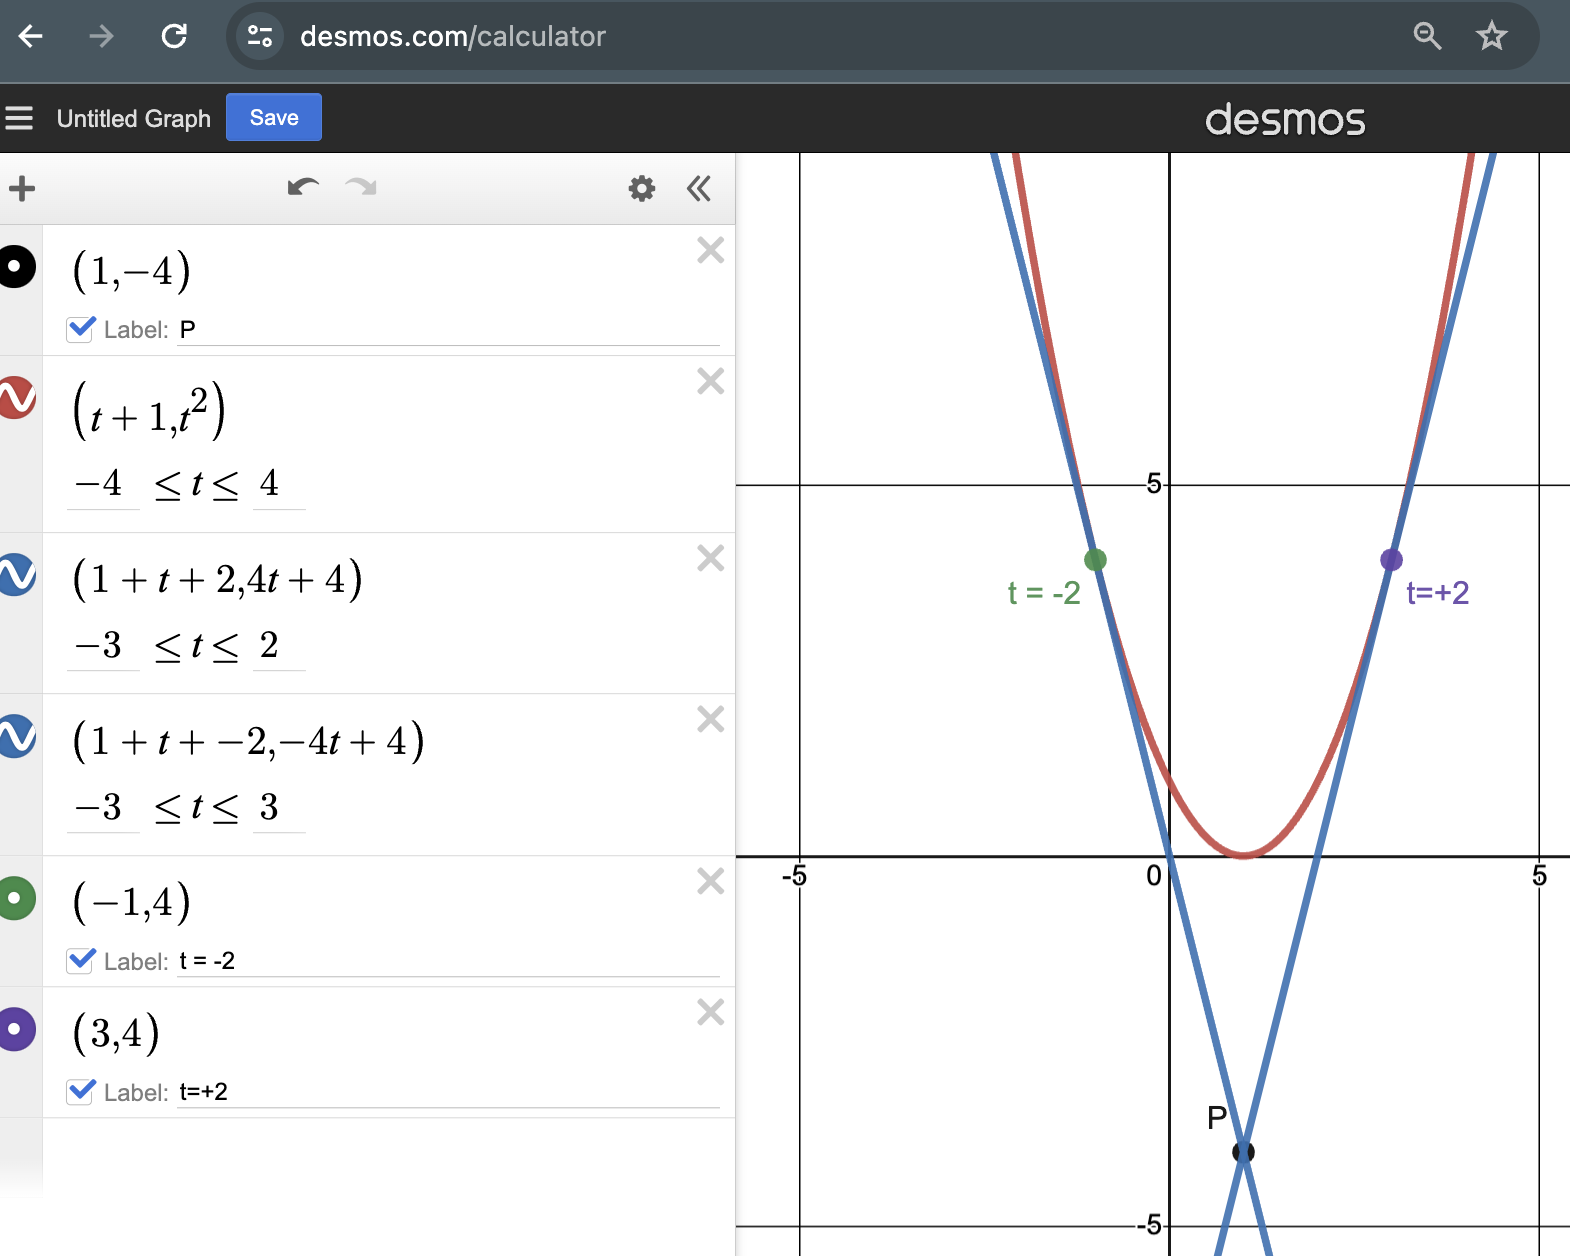
\includegraphics[width=0.75\paperwidth]{202402/Exam1/Images/Tangents.png}
    } 
    \else
      
    \fi        
\fi






\ifnum \Version=3
    \part The equation of the tangent line to the curve $\mathbf r(t) =\langle 1-t,t^2,3t\rangle$ at the point where $t=1$ has equation $\mathbf{L} = \langle f(t), g(t), g(t) \rangle$, where $f(t) = \framebox{\strut\hspace{2cm}}$, $g(t) = \framebox{\strut\hspace{2cm}}$, $h(t) =\framebox{\strut\hspace{2cm}}$.
    
    \ifnum \Solutions=1 {\color{DarkBlue} \textit{Solutions:} 
    The tangent line is parallel to $r'(t)$.
    \begin{align}
        \mathbf r'(t) &= \langle -1,2t,3\rangle \\
        \mathbf r'(1) &= \langle -1,2,3\rangle 
    \end{align}
    And $\mathbf r(1) = \langle 0,1,3\rangle$. Therefore, $\mathbf L(t) = \langle 0-t, 1 +2t, 3+3t\rangle$.
    } 
    \else
      
    \fi        
\fi

\ifnum \Version=4
    \part The position of a moving object is given by the curve $\mathbf r(t) = \langle 1-t^2,t^3\rangle$ for $t\in \mathbb R$. The value of $t$ that corresponds to the time when the direction of motion is parallel to $\mathbf w = \langle -2, 6\rangle$, is $t = \framebox{\strut\hspace{1cm}}$. 
    
    \ifnum \Solutions=1 {\color{DarkBlue} \textit{Solutions:} 
    The direction of motion is parallel to the velocity. 
    \begin{align}
        \mathbf r'(t) = \mathbf v &= \langle -2t,3t^2\rangle 
    \end{align}
    Vectors are parallel when they are non-zero multiples of each other. So the velocity will be parallel to the given $\mathbf w$ vector when they are non-zero multiples of each other. If we let $\lambda \ne 0$ be the multiple, then we can solve
    \begin{align}
        \mathbf v &= \lambda \mathbf w \\
        \begin{pmatrix} -2t  \\ 3t^2 \end{pmatrix} &= \lambda \begin{pmatrix} -2\\6 \end{pmatrix}
    \end{align}
    The first components give us $t=\lambda$. The second components give us
    \begin{align}
        3t^2 = 6\lambda
    \end{align}
    But $\lambda = t$, so we have
    \begin{align}
        3t^2 &= 6t \\
        t(t-2) &= 0
    \end{align}  
    So the values of $t$ that satisfy $\mathbf v = \lambda \mathbf w$ are $t=0$ and $t=2$. But $\mathbf r(0)$ is not parallel to $\mathbf w$. So the only value of $t$ where the two vectors are parallel is $t=2$. 
    } 
    \else
    \fi        
\fi


\ifnum \Version=5
    \part The equation of the tangent line to the curve $\mathbf r(t) =\langle t-1,3t,t^2\rangle$ at the point where $t=2$ has equation $\mathbf{L} = \langle f(t), g(t), g(t) \rangle$, where $f(t) = \framebox{\strut\hspace{2cm}}$, $g(t) = \framebox{\strut\hspace{2cm}}$, $h(t) =\framebox{\strut\hspace{2cm}}$.
    
    \ifnum \Solutions=1 {\color{DarkBlue} \textit{Solutions:} The tangent line is parallel to $r'(t)$.
    \begin{align}
        \mathbf r'(t) &= \langle 1,3,2t\rangle \\
        \mathbf r'(2) &= \langle 1,3,4\rangle 
    \end{align}
    And $\mathbf r(2) = \langle 1,6,4\rangle$. Therefore, $\mathbf L(t) = \langle 1+t, 6 + 3t, 4+4t\rangle$.
    
    } 
    \else
    \fi        
\fi



\ifnum \Version=6


\part The tangent line to the curve $\mathbf r(t) =\langle 4t-1,t^3,t^2\rangle$ at the point where $t=2$ is $\mathbf{L} = \langle f(t), g(t), g(t) \rangle$, where $f(t) = \framebox{\strut\hspace{2cm}}$, $g(t) = \framebox{\strut\hspace{2cm}}$, $h(t) =\framebox{\strut\hspace{2cm}}$.

\ifnum \Solutions=1 {\color{DarkBlue} \textit{Solutions:} The tangent line is parallel to $r'(t)$.
\begin{align}
    \mathbf r'(t) &= \langle 4,3t^2,2t\rangle \\
    \mathbf r'(2) &= \langle 4,12,4\rangle 
\end{align}
And $\mathbf r(2) = \langle 7, 8,4\rangle$. Therefore, $\mathbf L(t) = \langle 7+4t, 8+12t,4+4t\rangle$.

} 
\else
  
\fi        
\fi







\ifnum \Version=7
    \part The position of a moving object is given by the curve $\mathbf r(t) = \langle 2+t,4,t^2\rangle$ for $t\in \mathbb R$. The speed of the object at $t=2$ is $\framebox{\strut\hspace{2cm}}$. A unit vector that gives the direction of motion at time $t=2$ is $\mathbf T = \langle f(t), g(t), h(t)\rangle$, where $f = \framebox{\strut\hspace{1.75cm}}$, $g = \framebox{\strut\hspace{1.75cm}}$, $h= \framebox{\strut\hspace{1.75cm}}$. 
    
    \ifnum \Solutions=1 {\color{DarkBlue} \textit{Solutions:} 
    The speed is the magnitude of the velocity. 
    \begin{align}
        \mathbf r'(t) = \mathbf v &= \langle 1,0,2t \rangle \\
        | \mathbf r'(t) | &= \sqrt{1+4t^2} \\
        | \mathbf r'(2) | &= \sqrt{1+16} = \sqrt{17}
    \end{align}
    We can write the speed as $\sqrt{17}$. We do not need to express the answer using any units. The unit tangent vector $\mathbf T$ gives the direction of motion at any time $t$. 
    \begin{align}
        \mathbf T 
        &= \frac{\mathbf r'(t)}{| \mathbf r'(t) |} 
        = \left\langle 
        \frac{1}{\sqrt{1+4t^2\, }},
        0,
        \frac{2t}{\sqrt{1+4t^2\,}}
        \right\rangle
    \end{align}
    Therefore,
    \begin{align}
        f(2) &= \frac{1}{\sqrt{1+4(2)^2\, }} = \frac{1}{\sqrt{17}}\\
        g(2) &= 0\\
        h(2) &= \frac{2(2)}{\sqrt{1+4(2)^2\,}} = \frac{4}{\sqrt{17}}
    \end{align}
    No further simplification needed. But it is also ok to write the answer as
    \begin{align}
        f(2) &= \frac{\sqrt{17}}{17}\\
        g(2) &= 0\\
        h(2) &= \frac{4\sqrt{17}}{17}
    \end{align}    
    } 
    \else
      
    \fi        
\fi




\ifnum \Version=8
    \part The position of a moving object is given by the curve $\mathbf r(t) = \langle 1-2t,6t^3\rangle$ for $t\in \mathbb R$. The curve passes through the point $P(5,-48)$ when $t = \framebox{\strut\hspace{1cm}}$. The times when the direction of motion is perpendicular to $\mathbf w = \langle 1, 1\rangle$, are $t = \framebox{\strut\hspace{1cm}}$ and $t = \framebox{\strut\hspace{1cm}}$. 
    
    \ifnum \Solutions=1 {\color{DarkBlue} \textit{Solutions:} The point will be at $P$ when 
    \begin{align}
        \mathbf r (t) = \langle 1 - 2t, 6t^3 \rangle = \langle 5, - 48 \rangle
    \end{align}
    Solving for $t$ we see that $t = -2$. The direction of motion is parallel to the velocity. 
    \begin{align}
        \mathbf r'(t) = \mathbf v &= \langle -2,18t^2\rangle 
    \end{align}
    Vectors are perpendicular when their dot products are zero. So the velocity will be orthogonal to the given $\mathbf w$ vector when
    \begin{align}
        0 &= \mathbf v \cdot \mathbf w 
        = \begin{pmatrix} -2  \\ 18t^2 \end{pmatrix} \cdot \begin{pmatrix} 1\\1 \end{pmatrix} = -2 + 18t^2 \\
        &= 9t^2 - 1 \\
        t &= \pm 1/3
    \end{align}
    } 
    \else
    \fi        
\fi


\ifnum \Version=9


\part Suppose that the tangent line to the curve $\mathbf r(t) = \langle 2t-1,t-3,2t^2\rangle$ at the point where $t=t_0=3$ is $\mathbf{L} = \langle f(u), g(u), g(u) \rangle$, $u \in \mathbb R$. Then the parametric equations for the tangent line at $t_0$, with parameter $u$, are $f(u) = \framebox{\strut\hspace{2cm}}$, $g(u) = \framebox{\strut\hspace{2cm}}$, $h(u) =\framebox{\strut\hspace{2cm}}$. The curve intersects the plane $x+2y=4$ when $t = \framebox{\strut\hspace{1cm}}$. 

\ifnum \Solutions=1 {\color{DarkBlue} \textit{Solutions:} The tangent line is parallel to $\mathbf r'(t)$.
\begin{align}
    \mathbf r'(t) &= \langle 2,1,4t\rangle \\
    \mathbf r'(3) &= \langle 2,1,12\rangle 
\end{align}
And $\mathbf r(3) = \langle 2,1,18\rangle$. Therefore, $\mathbf L(u) = \langle 2+2u,1+u,18+12u\rangle$.

The curve intersects the plane when the components of the curve satisfy the plane equation. 
\begin{align}
    4 &= x+y+z = 2t-1 + 2(t-3) = 4t -4 \\
    8 &= 4t
\end{align}
The point corresponds to $t=2$. 
} 
\else
  
\fi        
\fi

\ifnum \Version=10
    \part The position of a moving object is given by the curve $\mathbf r(t) = \langle 1-t,4,3t\rangle$ for $t\in \mathbb R$. The speed of the object is given by $\framebox{\strut\hspace{2cm}}$. A unit vector that gives the direction of motion at time $t$ is $\mathbf T = \langle f(t), g(t), h(t)\rangle$, where $f = \framebox{\strut\hspace{1.75cm}}$, $g = \framebox{\strut\hspace{1.75cm}}$, $h= \framebox{\strut\hspace{1.75cm}}$. 
    
    \ifnum \Solutions=1 {\color{DarkBlue} \textit{Solutions:} 
    The speed is the magnitude of the velocity. 
    \begin{align}
        \mathbf r'(t) = \mathbf v &= \langle -1,0,3 \rangle \\
        | \mathbf r'(t) | &= \sqrt{1+1+(6t)^2} = \sqrt{1+0+3^2} = \sqrt{10}
    \end{align}
    We can write the speed as $\sqrt{10}$. We do not need to express the answer using any units. The unit tangent vector $\mathbf T$ gives the direction of motion at any time $t$. 
    \begin{align}
        \mathbf T 
        &= \frac{\mathbf r'(t)}{| \mathbf r'(t) |} 
        = \left\langle 
        \frac{-1}{\sqrt{10}},
        0,
        \frac{3}{\sqrt{10}}
        \right\rangle
    \end{align}
    Therefore,
    \begin{align}
        f &= -1 / \sqrt{10} \\
        g &= 0\\
        h &= 3 / \sqrt{10}
    \end{align}
    No further simplification needed. 
    } 
    \else
      
    \fi        
\fi